\section{Further Expression}
\hspace*{0.5in} Setiap kode yang dituliskan menggunakan bahasa yang dikompilasi seperti C, C++ atau Java dapat diintegrasikan ke skrip Python lainnya. Kode ini dianggap sebagai ektensi. 

\hspace*{0.5in} Modul ekstensi Python tidak lebih dari sekedar perpustakaan C biasa. Pada mesin Unix, perpustakaan ini biasanya diakhiri dengan .so (untuk objek bersama). Pada mesin windows, biasanya melihat .dll (untuk perpusatkaan yang terhubung secara dinamis).  


\subsection{Pra-Persyaratan untuk Menulis Ekstensi} 

\hspace*{0.5in} Untuk memulai ektensi, memerlukan file header Python. Pada mesin Unix, biasanya memerlukan instalasi paket khusus pengembang seperti python 2-5. 

\hspace*{0.5in} Pengguna window mendapatkan header ini sebagai bagian dari paket saat menggunakan pemasang Python biner. 

\hspace*{0.5in} Harus memiliki pengetahuan yang baik tentang C atau C++ untuk menulis ekstensi Python menggunakan pemrograman C. 
 
\hspace*{0.5in} Untuk melihat modul ekstensi Python, perlu mengelompokkan kode menjadi empat bagian : 

\begin{itemize}
\item File header Python 
\item Fungsi C yang ingin ditampilkan sebagai antarmuka dari modul 
\item Sebuah tabel memetakan nama-nama fungsi saat pengembang Python melihat ke fungsi C didalam modul ekstensi 
\item Fungsi inilisasi
\end{itemize}
 
\vspace{12pt}
\hspace*{0.5in} Perlu menyertakan file header Python.h di file sumber C memberi akses ke API Python internal digunakan untuk menghitung modul ke penerjamah. 
Menyertakan header Python.h sebelum header lain yang mungkin dibutuhkan. Mengikuti termasuk dengan fungsi yang ingin dipanggil dari Python. 
Tanda tangan penerapan C fungsi selalu mengambil salah satu dari tiga bentuk berikut : 


\begin{verbatim}
static PyObject *MyFunction( PyObject *self, PyObject *ar
gs);} 
 
static PyObject *MyFunctionWithKeywords(PyObject *self,} 

                                        PyObject *args,} 

                                        PyObject *kw);} 
                                        
static PyObject *MyFunctionWithNoArgs( PyObject *self );} 
\end{verbatim}

\vspace{12pt}
\hspace*{0.5in} Masing-masing deklarasi seelumnya mengembalikan objek Python. Tidak ada yang namanya fungsi void dengan Python seperti ada di C. Jika ingin fungsi mengembalikan nilai, Python. Header Python mendefinisikan makro.  

\hspace*{0.5in} Nama-nama fungsi C bisa menjadi apapun yang disuka karena tidak pernah diluar modul ekstensi mendefinisikan sebagai statis. 

\hspace*{0.5in} Fungi Cbiasanya diberi nama dengan menggabnungkan modul dan fungsi Python bersama-sama yang ditunjukan disini : 


\begin{verbatim}
static PyObject *{module $  \_  $func}(PyObject *self, 
PyObject *args) $ \{ $ 

    /* Do your stuff here. */ 

    Py $  \_  $RETURN $  \_  $NONE; 

 $  \}  $ 
\end{verbatim}

\vspace{12pt}
\hspace*{0.5in} Ini adalah fungsi Python yang disebut func didalam modul-modul. Memasukkan petunjuk ke fungsi C ke dalam tabel metode untuk modul yang biasanya muncul selanjutnya dikode sumber tael pemetaan metode. 

\hspace*{0.5in} Tabel metode ini adalah susunan sederhana dari struktur PyMethodSef. Struktur itu terlihat seperti ini : 

\begin{verbatim}
struct PyMethodDef  $  \{  $ 
 
   char *ml $  \_  $name; 
 
   PyCFunction ml $  \_  $meth; 

   int ml $  \_  $flags; 
 
   char *ml $  \_  $doc; 

 $  \}  $; 
\end{verbatim}

\vspace{12pt}
Ini nilai uraian anggota struktur ini : 

\begin{itemize}
\item Ml $  \_  $name 

Nama fungsi yang digunakan penafsir Python saat digunakan dalam program Python 
\item Ml $  \_  $meth 

Menjadi alamaat ke fungsi yang memiliki salah satu tanda tangan yang dijelaskan dalam penelusuran sebelumnya 
\item Ml $  \_  $flags 

Memberitahu penafsir yang mana dari tiga tanda tangan yang digunakan ml $  \_  $meth. Bendera ini biasanya mmiliki nilai meth $  \_  $varargs. Bendera ini dapat digandakan dengan or’ed dengan meth $  \_  $keywords jika ingin memiarkan argumen kata kunci masuk ke fungsi. Ini juga bisa memiliki nilai meth $  \_  $noargs yang menunjukan bahwa tidak ingin menerima argumen apa pun. 
\item Ml $  \_  $doc 

Ini adalah docstring untuk fungsi yang bisa jadi NULL jika tidak ingin menulisnya. 
\vspace{12pt}

\hspace*{0.5in} Tabel ini perlu diakhiri dengan sentinel yang terdiri dari NULL dan 0 untuk anggota yang sesuai. 
\vspace{12pt}

Contoh: 
\begin{verbatim}
static PyMethodDef {module} $  \_  $methods[] 
=  $  \{  $ 

   $  \{  $ "{func}", (PyCFunction){module $
\_  $func}, METH $  \_  $NOARGS, NULL  $  \}  $, 

   $  \{  $ NULL, NULL, 0, NULL  $  \}  $ 

 $  \}  $; 
\end{verbatim}

\vspace{12pt}
\hspace*{0.5in} Bagian terakhir dari modul ekstensi adalah fungsi inialisasi. Fungsi ini dipanggil oleh juru bahasa Python saat modul diisikan. Hal ini diperlukan agar fungsi diberi nama intiModule dimana modul adalah nama modul. 

\hspace*{0.5in} Fungsi inialisasi perlu diekspor dari perpustakaan yang akan dibangun. Header Python mendefinisikan PyMODINIT $  \_  $Func untuk memasukkan mantra yang sesuai agar terjadi pada lingkungan tertentu tempat menyuusun. Yang harus dilakukan adalah mengunakan saat menentukan fungsinya. Fungsi inialisasi C umumnya memiliki strktur keseluruhan berikut : 
\begin{verbatim}
PyMODINIT $  \_  $FUNC init{Module}()  $  \{  $ 

   Py $  \_  $InitModule3({func}, {module} $  \_ 
   $methods, "docstring..."); 

 $  \}  $ 
\end{verbatim}

\vspace{12pt}
Berikut adalah penjelasan fugsi Py $  \_  $IntiModule : 
\item Func  

Ini adalah fungsi yang akan diekspor 
\item Module 

Ini adalah nama tabel pemetaan yang didefinisikan diatas 
\item Docstring

Ini adalah komentar yang ingin diberikan diekstensi 
\end{itemize}

\vspace{12pt}
Menempatkan ini semua bersama-sama terlihat sebagai berikut : 
\begin{verbatim}
 $  \#  $include <Python.h>

static PyObject *{module $  \_  $func}(PyObject *self, 
PyObject *args)  $  \{  $ 

   /* Do your stuff here. */ 

   Py $  \_  $RETURN $  \_  $NONE; 

 $  \}  $ 
 
static PyMethodDef {module} $  \_  $methods[] =  $ 
\{  $ 

    $  \{  $ "{func}", (PyCFunction){module $  \_ 
    $func}, METH $  \_  $NOARGS, NULL  $  \}  $, 
 
    $  \{  $ NULL, NULL, 0, NULL  $  \}  $ 

 $  \}  $; 

PyMODINIT $  \_  $FUNC init {Module}()  $  \{  $ 
 
   Py $  \_  $InitModule3({func}, {module} $  \_ 
   $methods, "docstring..."); 

 $  \}  $ 
\end{verbatim}

\vspace{12pt}
Contoh: 
\begin{verbatim} 
 $  \#  $include <Python.h> 
 
static PyObject* helloworld(PyObject* self) 

 $  \{  $ 
 
   return Py $  \_  $BuildValue("s", "Hello, Python 
   extensions!!"); 

 $  \}  $ 
 
static char helloworld $  \_  $docs[] = 
static PyMethodDef helloworld $  \_  $funcs[] =  $  
\{  $ 

    $  \{  $"helloworld", (PyCFunction)helloworld,  

    METH $  \_  $NOARGS, helloworld $  \_  $docs $  
    \}  $, 

    $  \{  $NULL $  \}  $
 
 $  \}  $; 
 
void inithelloworld(void) 
 
 $  \{  $ 

   Py $  \_  $InitModule3("helloworld", helloworld $  
   \_  $funcs, 

             "Extension module example!"); 
 
 $  \}  $ 
\end{verbatim}

\vspace{12pt} 
\hspace*{0.5in} Disini fungsi Py $  \_  $BuildValue digunakan untuk membangun nilai Python.  

\vspace{12pt} 
\subsection{Membangun dan Menginstal Ekstensi} 

\hspace*{0.5in} Paket membuatnya sangat mudah mendistribusikan modul Python, baik Python murni dan modul ekstensi dengan cara standar. Modul didistribusikan dalam bentuk sumber dan dibangun dan diinstal melalui skrip setup yang iasa disebut setup.py sebagai berikut : 
 
\begin{verbatim}
from distutils.core import setup, Extension \par
      ext $  \_  $modules=[Extension('helloworld', 
      ['hello.c'])]). 
\end{verbatim}

\vspace{12pt}
\hspace*{0.5in} Sekarang gunakan perintah berikut yang aka melalakukan semua kompilasi dan langkah penghubunh yang diperlukan dengan perintah dan bendera penyusun dan penghubung yang benar dan menyalin perpustakaan dinamis yang dihasilkan ke dalam direktori yang sesuai . 
\vspace{12pt}
 
Contoh : 
\begin{verbatim}
$  \$  $ python setup.py install
\end{verbatim}
  
\vspace{12pt}
\hspace*{0.5in} Pada sistem berbasis Unix kemungkinan besar perlu menjalankan perintah ini sebagai root agar meminta izin untuk menulis ke direktori paket situs. Ini biasanya tidak menjadi masalah pada window. 
Setelah~menginstal ekstensi, akan dapat mengimpor dan memanggil ekstensi tersebut di skrip Python  sebagai berikut : 
\begin{verbatim}
$  \#  $!/usr/bin/python

  import helloworld 

  print helloworld.helloworld() 
\end{verbatim}

\vspace{12pt}
Ini akan menghasilkan hasil sebagai berikut  : 
Hello, Python extensions!! 

\vspace{12pt}
Seperti kemungkinan besar ingin mendefinisikan fungsi yang menerima argumen, dapat menggunakan salah satu tanda tangan lain untuk fungsi C. Sebagai contoh, fungsi berikut yang menerima beberapa parameter akan didefinisikan seperti ini : 
\begin{verbatim}
static PyObject *{module $  \_  $func}(PyObject 
*self, PyObject *args)  $  \{  $ 

    /* Parse args and do something interesting here. */ 

    Py $  \_  $RETURN $  \_  $NONE; 

 $  \}  $ 
\end{verbatim}

\vspace{12pt}
Tabel metode yang berisi entri untuk fungsi baru akan terlihat seperti ini : 
\begin{verbatim}
static PyMethodDef {module} $  \_  $methods[] =  $  
\{  $ 

    $  \{  $ "{func}", (PyCFunction) {module
    $  \_  $func}, METH $  \_  $NOARGS, NULL  $  \}  $, 

    $  \{  $ "{func}", {module $  \_  $func
    }, METH $  \_  $VARARGS, NULL  $  \}  $, 

    $  \{  $ NULL, NULL, 0, NULL  $  \}  $ 

 $  \}  $; 
\end{verbatim}

\vspace{12pt}
Menggunakan fungsi API PyArg $  \_  $ParseTuple untuk mengekstrak argumen dari satu pointer PyObject yang dikirimkan ke fungsi C. Argumen pertama untuk PyArg $  \_  $ParseTuple adalah args argumen. Ini adalah objek yang akan parsing. Argumen kedua adalah string format yang menggambarkan argumen saat mengharapkannya muncul. Setiap argumen diwakili oleh satu atau lebih karakter dalam format string sebagai berikut : 

\begin{verbatim}
static PyObject *{module $  \_  $func}(PyObject *self, 
PyObject *args)  $  \{  $ 

    int i;

   double d; 

   char *s; 
   
   if (!PyArg $  \_  $ParseTuple(args, "ids",  $  \&  $i,
   $  \&  $d,  $  \&  $s))  $  \{  $ 

   return NULL; 

   $  \}  $ 

   /* Do something interesting here. */ 

   Py $  \_  $RETURN $  \_  $NONE; 

   $  \}  $ 
\end{verbatim}

\vspace{12pt}
Mengkompilasi versi baru dari modul dan mengimpornya memungkinkan untuk memanggil fungsi baru dengan sejumlah argumen dari jenis apa pun : 
\begin{verbatim}
module.func(1, s="three", d=2.0) 

module.func(i=1, d=2.0, s="three") 

module.func(s="three", d=2.0, i=1) 

\end{verbatim}
\vspace{12pt}
\hspace*{0.5in} Berikut adalah tanda tangan standar untuk 
fungsi PyArg $  \_  $ParseTuple: 
 
\begin{verbatim}
int PyArg $  \_  $ParseTuple(PyObject* tuple,char* format,...) 
\end{verbatim}

\vspace{10pt}
\hspace*{0.5in} Fungsi ini mengembalikan 0 untuk kesalahan, dan nilai tidak sama dengan 0 untuk kesuksesan. Tuple adalah PyObject * yang merupakan argumen kedua dari fungsi C. Format berikut adalah string C yang menggambarkan argumen wajib dan opsional. Berikut adalah daftar kode format untuk fungsi PyArg $  \_  $ParseTuple: 

 %%%%%%%%%%%%  Table No:1 Here %%%%%%%%%%%%%%


\begin{table}[ht]
	\caption{Ukuran}
	\begin{tabular*}{\textwidth}{@{\extracolsep{\fill}}lcc}
		\hline
		Karakter&  Penjelasan \cr
		\hline
		c&Sentimeter&\cr
		i&Inci&\cr
		m&Milimeter&\cr
		p&Poin printer\cr
		\hline
	\end{tabular*}
	\begin{tablenotes}
	\end{tablenotes}
\end{table}

%%%%%%%%%%%%  Table No:1 Ends Here %%%%%%%%%%%%%%

\vspace{80pt}
Py $  \_  $BuildValue~mengambil format string seperti PyArg $  \_  $ParseTuple. Alih-alih menyampaikan alamat nilai yang sedang  bangun, melewati nilai sebenarnya. Berikut adalah contoh yang menunjukkan bagaimana menerapkan fungsi tambah : 

\begin{verbatim}
static PyObject *foo $  \_  $add(PyObject *self, PyObject 
*args)  $  \{  $ 

   int a; 

   int b; 
\vspace{12pt}

   if (!PyArg $  \_  $ParseTuple(args, "ii",  $  \&  $a,
   $  \&  $b))  $  \{  $ 

    return NULL;

    $  \}  $ 

    return Py $  \_  $BuildValue("i", a + b); 

 $  \}  $ 

 def add(a, b):

 return (a + b) 

 static PyObject *foo $  \_  $add $  \_  $subtract(PyObject 
 *self, PyObject *args)  $  \{  $ 

  int a; 

  int b; 

  if (!PyArg $  \_  $ParseTuple(args, "ii",  $  \&  $a,  $  
  \&  $b))  $  \{  $ 

  return NULL; 

  $  \}  $ 

  return Py $  \_  $BuildValue("ii", a + b, a - b); 

 $  \}  $ 

  def add $  \_  $subtract(a, b): 

  return (a + b, a - b) 
\end{verbatim}  

\vspace{10pt}
Berikut daftar tabel string kode yang umum digunakan, yang nol atau lebihnya digabungkan ke dalam format string : 


 %%%%%%%%%%%%  Table No:2 Here %%%%%%%%%%%%%%


\begin{table}[ht]
	\caption{Ukuran}
	\begin{tabular*}{\textwidth}{@{\extracolsep{\fill}}lcc}
		\hline
		Code& C Type&  Meaning\cr
		\hline
		c&char&String Python dengan panjang 1 menjadi huruf C.\cr
		d&double&Pelampung Python menjadi C ganda.\cr
		f&float&Pelampung Python menjadi pelampung C.\cr
		i&int&Int Python menjadi int int\cr
		l&long&Sebuah int Python menjadi panjang C.\cr
		L&long long&Sebuah int Python menjadi C panjang panjang\cr
		O&PyObject*&Gets non-NULL meminjam referensi ke argumen Python\cr
		s&char*&Python string tanpa nulls tertanam ke C char *\cr
		s&char*+int&Setiap string Python ke alamat dan panjang C\cr
		t&char*+int&Read-only penyangga segmen tunggal ke alamat C dan panjangnya\cr
		U&PyUNICODE*&Python Unicode tanpa nulls tertanam ke C\cr
		u&PPyUNICODE*int+&Setiap alamat dan panjang Python Unicode C\cr
		w&char*+int&Membaca / menulis penyangga segmen tunggal ke alamat dan panjang C\cr
		Z&char*&Seperti s, juga menerima None (set C char * ke NULL).\cr
		z&char*+int&Seperti s, juga menerima None set C char * ke NULL\cr
		(...)&Poin printer&Urutan Python diperlakukan sebagai satu argumen per item.\cr
		|&as per ...&Argumen berikut bersifat opsional.\cr
		:&&Format akhir, diikuti dengan nama fungsi untuk pesan error.\cr
		;&&Format akhir, diikuti oleh seluruh pesan kesalahan teks.\cr				
		\hline
	\end{tabular*}
	\begin{tablenotes}
	\end{tablenotes}
\end{table}


 %%%%%%%%%%%%  Table No:2 Ends Here %%%%%%%%%%%%%%


\vspace{12pt}
Kode  $  \{  $... $  \}  $ membangun kamus dari sejumlah nilai C, kunci dan nilai bergantian. Misalnya, Py $  \_  $BuildValue (" $  \{  $issi $  \}  $", 23, "zig", "zag", 42) mengembalikan kamus seperti  $  \{  $23: 'zig', 'zag': 42 $  \}  $ Python. Setiap blok memori yang dialokasikan dengan malloc () pada akhirnya harus dikembalikan ke genangan memori yang tersedia dengan satu panggilan untuk membebaskan (). Penting untuk menelepon gratis () pada waktu yang tepat. Jika alamat blok dilupakan tapi gratis () tidak dipanggil untuk itu, memori yang ditempatinya tidak dapat digunakan kembali sampai program berakhir. Ini disebut kebocoran memori. Di sisi lain, jika sebuah program memanggil gratis () untuk satu blok dan kemudian terus menggunakan blok tersebut, itu menciptakan konflik dengan penggunaan ulang blok melalui panggilan malloc () yang lain. Ini disebut dengan menggunakan memori yang dibebaskan. Ini memiliki konsekuensi buruk yang sama seperti merujuk pada data yang tidak diinisiasi - dump inti, hasil yang salah, crash misterius. Karena Python membuat penggunaan malloc () dan gratis (), dibutuhkan strategi untuk menghindari kebocoran memori dan juga penggunaan memori yang bebas. Metode yang dipilih disebut penghitungan referensi. Prinsipnya sederhana: setiap objek berisi sebuah counter, yang bertambah saat referensi ke objek disimpan di suatu tempat, dan yang dikurangi saat referensi itu dihapus. Saat counter mencapai nol, referensi terakhir ke objek telah dihapus dan objeknya dibebaskan. 

\section{Simbol Further Expression}
\hspace*{0.5in} Simbol khusus yang paling penting adalah garis miring terbalik yang digunakan untuk dua tujuan. Pertama, backslash dapat digunakan untuk membuat lebih banyak karakter meta dalam ekspresi reguler. Kedua, jika simbol khusus diawali dengan garis miring terbalik, maka artinya khusus akan dihapus dan dengan demikian menghasilkan kecocokan literal dari simbol khusus tersebut.  Garis miring terbalik menciptakan beberapa masalah karena merupakan simbol khusus dengan ekspresi Python dan juga string Python. Ekspresi hanya akan menghasilkan kecocokan untuk \t. Untuk mengatasi masalah ini, ekspresi Python menggunakan notasi string mentah yang membuat ekspresi tetap sederhana. Dalam notasi string mentah, setiap string ekspresi diawali dengan r sehingga tidak perlu menambahkan backslash beberapa kali.Berikut \ref{SimbolFurhertExpression} SimbolFurhertExpression :
\vspace{12pt}

\begin{figure}[ht]
	\centerline{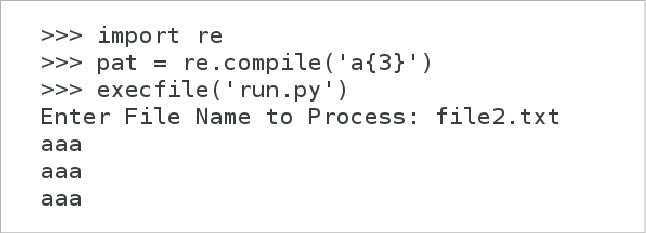
\includegraphics[width=0.50\textwidth]{figures/SimbolFurhertExpression}}
	\caption{SimbolFurhertExpression}
	\label{SimbolFurhertExpression}
\end{figure}

\vspace{12pt}
\hspace*{0.5in}Simbol adalah operator atau ekspresi biasa. Simbol khusus, tanda kurung tutup dan penutup, digunakan untuk mencari pola berulang. 